% =============================================================================
% Results (condensed to the IEEE conference length)
%
% Numbers are from committed results files produced on clean commits:
% results/forecasting.json (S1, d710cad), results/forecasting_wheeler.json (S6,
% 53ab76f), their re-runs (docs/RESULTS.md, Reproducibility check),
% results/forecasting_d21_p3.json (57e37aa), results/forecasting_d21_ablation_a1*.json
% and results/d21_tft_interpretation.json; D23 and D24 from
% results/forecasting_d23_e*.json (5ae2f84) and results/forecasting_d24_e*.json (947b33a); D25-D27 from
% results/forecasting_d25_e*.json (a59debb), results/forecasting_d26_e*.json (9866d7a) and
% results/forecasting_d27_e*.json (494b36f), D28 and D29 from results/forecasting_d28_e*.json (161c01f) and
% results/forecasting_d29_e*.json (f2fdd73), summarised in docs/RESULTS.md; table d26 is written
% from those files by hand. Other tables are generated by scripts/make_results_tables.py; figures by
% scripts/make_d25_d27_figures.py and scripts/make_d28_figures.py.
% =============================================================================

\section{Results}
\label{sec:results}

\emph{Data.} S1 diagnostics track the current SOH (median within-cell $\rho=0.97$ for the main incremental-capacity peak) but not the change to the next RPT (median $|\rho|\le0.3$); every S1 sample stays in class C0, while all S6 cells cross from C0 to C3.

% -----------------------------------------------------------------------------
\subsection{Continual stream (P1)}
\label{sec:res-p1}

% Generated by scripts/make_paper_tables.py from results/forecasting.json (commit d710cad), results/forecasting_wheeler.json (commit 53ab76f)
\begin{table*}[t]
  \centering
  \caption{Protocol P1 (continual stream). Final average test RMSE of SOH$(k{+}h)$ in pp (mean $\pm$ s.d.\ over 10 orders $\times$ 5 seeds for continual methods, over 5 seeds for joint training), skill relative to persistence ($1-\mathrm{RMSE}/\mathrm{RMSE}_{\mathrm{persistence}}$) and forgetting (pp). $^\dagger$Upper bound, trained on all tasks at once.}
  \label{tab:p1}
  \begin{tabular}{lccc|ccc}
    \toprule
    & \multicolumn{3}{c|}{S1: six NMC second-life cells} & \multicolumn{3}{c}{S6: 20 LFP cells, seven usage conditions} \\
    Method & RMSE & Skill & Forgetting & RMSE & Skill & Forgetting \\
    \midrule
    Persistence & 0.632 & 0.00 & -- & 1.644 & 0.00 & -- \\
    Linear extrapolation & 0.726 & -0.15 & -- & 0.343 & 0.79 & -- \\
    Ridge, usage only & 0.450 & 0.29 & -- & 1.274 & 0.22 & -- \\
    Ridge, F0 & 0.678 & -0.07 & -- & 0.801 & 0.51 & -- \\
    Ridge, F1 & 0.491 & 0.22 & -- & 0.605 & 0.63 & -- \\
    Gradient boosting, F1 & 0.466 & 0.26 & -- & 0.372 & 0.77 & -- \\
    \midrule
    MLP fine-tuning & 0.492 $\pm$ 0.029 & 0.22 & 0.030 & 0.531 $\pm$ 0.151 & 0.68 & 0.207 \\
    MLP replay & 0.475 $\pm$ 0.021 & 0.25 & 0.025 & 0.597 $\pm$ 0.178 & 0.64 & 0.212 \\
    MLP + EWC & 0.497 $\pm$ 0.033 & 0.21 & 0.040 & 0.540 $\pm$ 0.176 & 0.67 & 0.212 \\
    MLP joint$^\dagger$ & 0.500 $\pm$ 0.016 & 0.21 & -- & 0.414 $\pm$ 0.037 & 0.75 & -- \\
    \midrule
    TFT fine-tuning & 0.467 $\pm$ 0.014 & 0.26 & 0.026 & 0.883 $\pm$ 0.538 & 0.46 & 0.461 \\
    \textbf{TFT + EWC} & 0.462 $\pm$ 0.019 & 0.27 & 0.016 & 0.677 $\pm$ 0.261 & 0.59 & 0.274 \\
    TFT + EWC, F0 & 0.472 $\pm$ 0.020 & 0.25 & 0.019 & 0.621 $\pm$ 0.257 & 0.62 & 0.176 \\
    TFT joint$^\dagger$ & 0.455 $\pm$ 0.017 & 0.28 & -- & 0.427 $\pm$ 0.049 & 0.74 & -- \\
    \bottomrule
  \end{tabular}
\end{table*}


\emph{S1.} TFT\,+\,EWC reaches 0.462~pp (skill 0.27), level with gradient boosting, TFT fine-tuning and MLP replay (0.466--0.475~pp; Table~\ref{tab:p1}); a ridge regression on the planned usage alone is slightly better (0.450~pp). Forgetting is small for every method (0.016--0.040~pp). Differences whose significance changed in a re-run are only 0.005--0.014~pp (\S\ref{sec:res-repro}): on S1 the methods are practically equivalent.

\emph{S6.} When tasks differ in usage, forgetting is substantial (0.18--0.46~pp). EWC lowers the TFT's error and forgetting relative to fine-tuning (0.677 against 0.883~pp), but which difference is significant changed between runs (\S\ref{sec:res-repro}). MLP fine-tuning and MLP\,+\,EWC (0.531 and 0.540~pp) are significantly better in both runs, the joint upper bounds (0.414 and 0.427~pp) put the TFT's continual-learning cost at about 0.25~pp, and linear extrapolation (0.343~pp) and gradient boosting (0.372~pp) are the best forecasters. The TFT varies strongly with task order (s.d.\ 0.26~pp with EWC, 0.54~pp with fine-tuning).

% -----------------------------------------------------------------------------
\subsection{Unseen cell or usage condition (P2)}
\label{sec:res-p2}

% Generated by scripts/make_paper_tables.py from results/forecasting.json (commit d710cad), results/forecasting_wheeler.json (commit 53ab76f)
\begin{table}[t]
  \centering
  \caption{Protocol P2 (unseen battery in S1, unseen usage condition in S6): mean test RMSE (pp) over held-out groups, range over groups, and for S6 reuse-class accuracy / macro-F1 of the forecast SOH.}
  \label{tab:p2}
  \setlength{\tabcolsep}{3pt}
  \begin{tabular}{llccc}
    \toprule
    Data & Method & RMSE & Range & Class acc./F1 \\
    \midrule
    S1 & Persistence & 0.545 & 0.436--0.688 & -- \\
    S1 & Linear extrapolation & 0.511 & 0.284--0.725 & -- \\
    S1 & Ridge, usage only & 0.301 & 0.172--0.409 & -- \\
    S1 & Ridge, F0 & 0.418 & 0.158--0.779 & -- \\
    S1 & Ridge, F1 & 0.320 & 0.161--0.477 & -- \\
    S1 & Gradient boosting, F1 & 0.219 & 0.091--0.299 & -- \\
    S1 & MLP & 0.285 & 0.149--0.389 & -- \\
    S1 & TFT & 0.292 & 0.199--0.377 & -- \\
    \midrule
    S6 & Persistence & 2.817 & 2.025--4.327 & 0.85 / 0.64 \\
    S6 & Linear extrapolation & 1.372 & 0.856--1.669 & 0.94 / 0.75 \\
    S6 & Ridge, usage only & 1.177 & 0.870--2.288 & 0.95 / 0.83 \\
    S6 & Ridge, F0 & 0.859 & 0.598--1.836 & 0.96 / 0.86 \\
    S6 & Ridge, F1 & 1.137 & 0.588--2.188 & 0.96 / 0.85 \\
    S6 & Gradient boosting, F1 & 0.710 & 0.395--1.839 & 0.97 / 0.88 \\
    S6 & MLP & 0.821 & 0.476--2.225 & 0.96 / 0.87 \\
    S6 & TFT & 0.868 & 0.551--2.390 & 0.96 / 0.88 \\
    \bottomrule
  \end{tabular}
\end{table}


Gradient boosting is best on both datasets (Table~\ref{tab:p2}). On S6 the 100\% depth-of-discharge condition is the hardest for every method (1.8--2.4~pp). With six or seven held-out groups, no difference with the TFT survives Holm correction.

The further metrics (D30, from a re-run within 0.0052~pp of Table~\ref{tab:p2}) give the same ranking: gradient boosting has the largest $R^2_\Delta$ (0.54 on S1, 0.74 on S6), while linear extrapolation adds nothing to persistence ($-1.31$ and $-0.05$). On S6 the learned models assign the measured reuse class to 95--97\% of samples (MCC 0.90--0.93), against 94\% (0.88) for linear extrapolation and 86\% (0.72) for persistence; the end-of-first-life decision does not separate the methods (AUC $\ge$0.998), as 69\% of S6 samples are below 80\%.

% -----------------------------------------------------------------------------
\subsection{Reproducibility of the comparisons}
\label{sec:res-repro}

P1 and P2 were re-run in a pinned environment on data rebuilt from the raw archives. Every baseline, every P2 result and the ranking of methods reproduced; the neural models moved by at most 0.059~pp. On S1, five Holm-corrected comparisons with TFT\,+\,EWC crossed $p=0.05$. On S6, validation selected EWC $\lambda=1000$ instead of 100 (a 0.008~pp tie), and the error advantage of TFT\,+\,EWC over fine-tuning moved from $p_{\mathrm{Holm}}=0.005$ to 0.060, while its reduction of forgetting moved from 0.050 to 0.008. These findings motivated the ten tuning orders, the one-standard-error rule and the replication rule used from P3 on. A D30 re-run of P2 on another platform reproduced every baseline exactly and moved the MLP and TFT by at most 0.027~pp per held-out group: neural training is deterministic per platform, not across platforms.

% -----------------------------------------------------------------------------
\subsection{First-life pretraining (P3)}
\label{sec:res-p3}

The pool has 36{,}711 samples (S6: 2{,}409); validation selected EWC $\lambda=0.01$ for the pretrained TFT. Under the replication rule, EWC and fine-tuning are practically equivalent for the pretrained TFT (differences of 0.015--0.017~pp); both backbones are better from scratch on average (TFT 0.401/0.415~pp against 0.509/0.591~pp pretrained with EWC, significant only in the replicate set); and linear extrapolation (0.343~pp) remains the most accurate method. The S6 stream does not degrade the pool test error (TFT\,+\,EWC: 3.280 to 3.148~pp), but there too the pretrained models trail extrapolation (3.001~pp): pretraining learns no first-life model worth transferring.

\emph{Why the TFT improved.} A post hoc ablation, repeated on the replicate seeds, explains why the TFT from scratch improves from 0.891~pp with the earlier inputs to 0.401~pp with the shared ones: dropping the 17 diagnostic features lowers the error by 0.17--0.35~pp and adding the calendar time between checks by 0.19--0.31~pp, both replicated at both learning rates ($p_{\mathrm{Holm}}\le0.002$). Its attention over the four previous origins is nearly uniform (0.24--0.26 per lag): the TFT makes little use of its history.
\label{sec:res-interp}

% -----------------------------------------------------------------------------
\subsection{Learned residual on linear extrapolation}
\label{sec:res-residual}

\begin{table}[t]
  \centering
  \caption{Learned residual, shift-adaptive EWC and literature baselines on S6 (stream from scratch): final average test RMSE (pp), mean over 50 runs, main / replicate seed sets, and forgetting (pp) for horizons 1--6. Below the line: single fits on all tasks (not continual) and extrapolation.}
  \label{tab:residual}
  \setlength{\tabcolsep}{2.5pt}
  \scriptsize
  \begin{tabular}{lccc}
    \toprule
    Method & E1: $h{=}1$--3 & E2: $h{=}1$--6 & Forgetting, E2 \\
    \midrule
    \textbf{TFT\,+\,EWC, residual} & \textbf{0.339 / 0.314} & \textbf{0.561 / 0.534} & \textbf{0.093 / 0.086} \\
    TFT\,+\,SA-EWC, residual & 0.343 / 0.321 & 0.548 / 0.564 & 0.066 / 0.084 \\
    TFT fine-tuning, residual & 0.347 / 0.337 & 0.673 / 0.612 & 0.282 / 0.220 \\
    TFT\,+\,EWC, direct & 0.504 / 0.487 & 0.802 / 0.835 & 0.135 / 0.166 \\
    MLP\,+\,EWC, residual & 0.374 / 0.366 & 0.659 / 0.694 & 0.205 / 0.225 \\
    BiLSTM\,+\,EWC, residual & 0.328 / 0.370 & 0.669 / 0.765 & 0.229 / 0.318 \\
    Transformer\,+\,EWC, residual & 0.360 / 0.366 & 0.609 / 0.705 & 0.129 / 0.198 \\
    TCN\,+\,EWC, residual & 0.466 / 0.408 & 0.812 / 0.756 & 0.345 / 0.268 \\
    \midrule
    Linear extrapolation & 0.343 & 0.485 & -- \\
    Gradient boosting & 0.451 & 0.898 & -- \\
    SVR, residual & 0.429 & 0.616 & -- \\
    GPR, direct & 1.374 & 2.073 & -- \\
    \bottomrule
  \end{tabular}
\end{table}

For the residual form~\eqref{eq:residual} (Table~\ref{tab:residual}), the pre-registered criterion, residual TFT\,+\,EWC beating linear extrapolation, was \emph{not} met: the two are practically equivalent for horizons 1--3 (differences of $-0.004$ and $-0.029$~pp), and for horizons 1--6 extrapolation is better on average ($+0.076$ and $+0.049$~pp, not replicated). Per horizon, extrapolation is better at $h=1$ and 2 (replicated), and the gap closes without reversing by $h=5$--6. Learning the residual does make the TFT competitive: it improves TFT\,+\,EWC over the direct form by 0.17~pp (E1) and 0.24--0.30~pp (E2) and puts it ahead of gradient boosting, all replicated. For horizons 1--6, where it forgets more, EWC lowers its forgetting from 0.28/0.22 to 0.09~pp and its backward transfer from 0.18/0.14 to 0.03~pp, replicated; its effect on the final error is not. For horizons 1--3, EWC and fine-tuning are practically equivalent.

\emph{Ageing-cycle inputs.} The 21 Spark-extracted inputs (Section~\ref{sec:spark}), added as pre-specified, make the residual TFT\,+\,EWC worse: 0.480/0.501 against 0.339/0.314~pp, and worse than linear extrapolation, both replicated.

% -----------------------------------------------------------------------------
\subsection{Shift-adaptive EWC and literature baselines}
\label{sec:res-d24}

The second pre-registered criterion, for SA-EWC (Table~\ref{tab:residual}), was \emph{not} met: the residual TFT with SA-EWC and with fixed $\lambda$ are practically equivalent in final error and forgetting for both horizon sets (differences of at most 0.03~pp), although the shift weights did vary (0.05--1.14), so the simpler fixed $\lambda$ is kept. For horizons 1--3, BiLSTM\,+\,EWC (direct, 0.323~pp, and residual) and the residual Transformer\,+\,EWC are practically equivalent to the residual TFT; for 1--6 it beats the residual BiLSTM and TCN (replicated; not the Transformer). Every single-fit regressor is worse than the residual TFT\,+\,SA-EWC (replicated), except the residual SVR for horizons 1--6.

% -----------------------------------------------------------------------------
\subsection{Shrinkage and intervals on the stream}
\label{sec:res-d25}

Shrinking the correction per horizon makes the residual TFT\,+\,EWC practically equivalent to extrapolation at every horizon (0.318/0.308 against 0.343~pp for horizons 1--3, 0.498/0.493 against 0.485~pp for 1--6), removing its replicated loss at $h=1$--2; the correction is turned down most at $h=1$ (Fig.~\ref{fig:d25}). Again the criterion was not met: it matches extrapolation but does not beat it. Its 90\% intervals are narrower than extrapolation's but under-cover (0.71--0.81, against 0.92--0.95), so the interval scores are equal (practically equivalent or not replicated). Pretraining the residual model on the first-life pool makes it worse for horizons 1--3 (by 0.22~pp, replicated) and does not help for 1--6.

\begin{figure}[t]
  \centering
  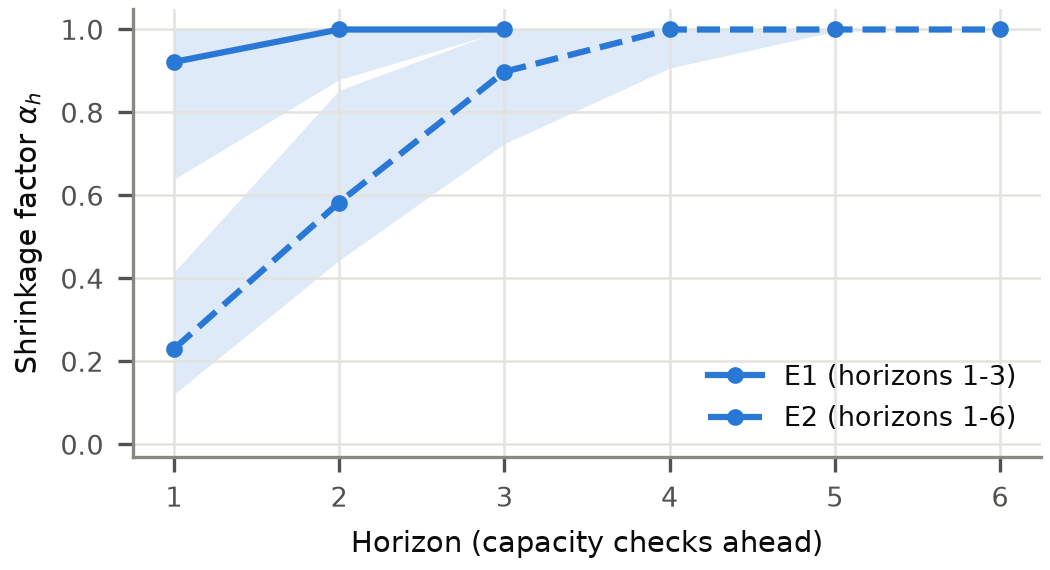
\includegraphics[width=\columnwidth]{figures/d25_shrinkage.png}
  \caption{S6 stream: shrinkage factor $\alpha_h$ of the TFT correction per horizon after the last task (median and interquartile range over 50 runs, seeds 0--4); $\alpha_h=0$ is linear extrapolation.}
  \label{fig:d25}
\end{figure}

% -----------------------------------------------------------------------------
\subsection{Residual model on unseen conditions}
\label{sec:res-d26}

\begin{table}[t]
  \centering
  \caption{Unseen S6 usage condition (P2, seven held-out conditions): test RMSE (pp), mean over folds, on all origins and on origins with a fade rate (H$^+$). TFT rows: mean over 50 runs, main / replicate seed sets; other rows: single deterministic fits.}
  \label{tab:d26}
  \setlength{\tabcolsep}{2.5pt}
  \scriptsize
  \begin{tabular}{lcccc}
    \toprule
    & \multicolumn{2}{c}{E1: $h{=}1$--3} & \multicolumn{2}{c}{E2: $h{=}1$--6} \\
    Method & all & H$^+$ & all & H$^+$ \\
    \midrule
    TFT\,+\,EWC, residual, shrunk & 0.92 / 0.94 & 0.74 / 0.74 & 1.62 / 1.65 & 1.42 / 1.44 \\
    TFT\,+\,EWC, residual, raw & 0.88 / 0.90 & 0.79 / 0.80 & 1.59 / 1.62 & 1.46 / 1.49 \\
    TFT, residual, joint & 0.57 / 0.58 & 0.54 / 0.55 & 1.21 / 1.18 & 1.22 / 1.19 \\
    \midrule
    Gradient boosting & \textbf{0.54} & \textbf{0.51} & \textbf{1.05} & \textbf{1.05} \\
    Ridge & 0.77 & 0.69 & 1.30 & 1.26 \\
    Linear extrapolation & 1.37 & 0.86 & 2.30 & 1.62 \\
    Persistence & 2.82 & 2.66 & 4.90 & 4.73 \\
    \bottomrule
  \end{tabular}
\end{table}

In the fourth experiment (Table~\ref{tab:d26}), as registered, the shrunk residual TFT\,+\,EWC beats extrapolation at origins with a fade rate, by 0.12/0.12~pp for horizons 1--3 and 0.20/0.18~pp for 1--6 (replicated): the first comparison in which the proposed model beats extrapolation. Elsewhere extrapolation is persistence and loses by over 2~pp. Gradient boosting, however, beats the TFT by 0.39/0.41~pp and 0.57/0.60~pp (replicated), on six of the seven conditions; only on the 100\% depth-of-discharge condition is the TFT better. The same residual TFT trained jointly on the six conditions beats its continual form by 0.32--0.44~pp (replicated). Shrinkage and the raw correction are practically equivalent here.

\begin{figure}[t]
  \centering
  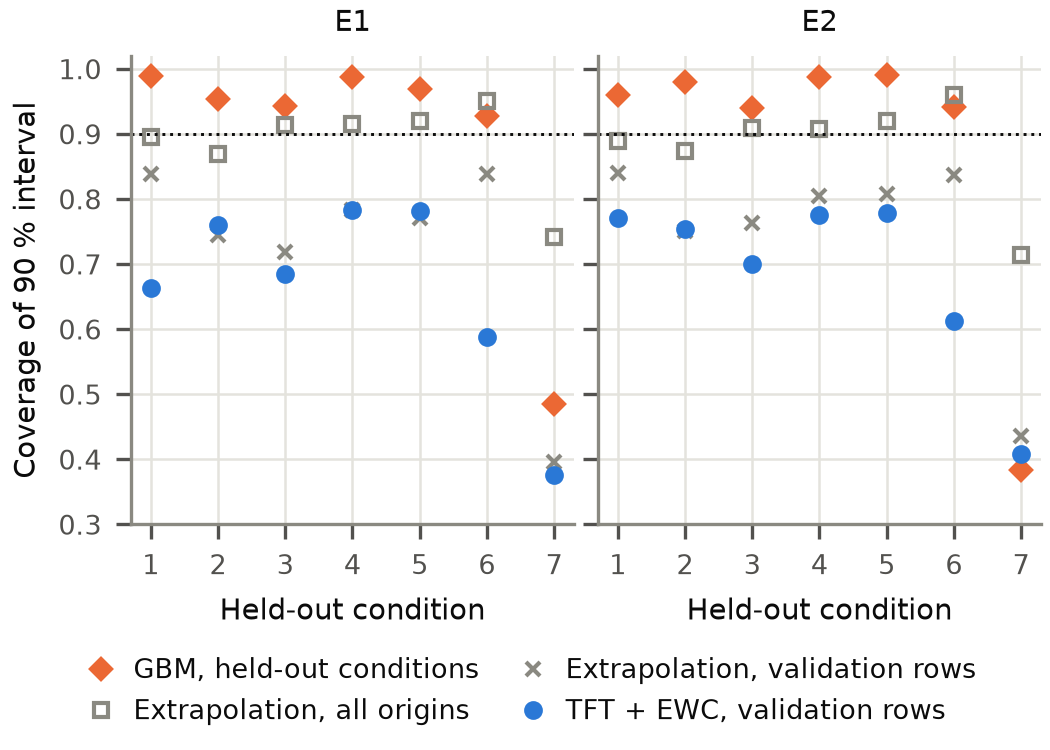
\includegraphics[width=\columnwidth]{figures/d27_coverage.png}
  \caption{Unseen S6 conditions: coverage of 90\% conformal intervals per held-out condition, by forecaster and calibration rows. TFT: mean over 50 runs (seeds 0--4). Dotted: nominal level.}
  \label{fig:d27}
\end{figure}

\emph{Intervals on unseen conditions.} Intervals (Fig.~\ref{fig:d27}) calibrated on the pooled validation rows of the training conditions under-cover on the held-out one, for the TFT (pooled 0.66--0.68) and for extrapolation (0.74--0.76) alike. Calibrating extrapolation, which has no fitted parameters, on all origins of those conditions instead of their mid-life validation rows restores 0.89--0.90: the calibration rows caused the shortfall, not only the model. With leave-one-condition-out calibration, gradient-boosting intervals reach the registered threshold of 0.85 (0.90 in both horizon sets) with the lowest mean interval scores (3.2 and 6.7~pp, against 7.1 and 11.8~pp for calibrated extrapolation and 6.1--6.3 and 10.0--10.3~pp for the TFT), lower than calibrated extrapolation's on six of seven conditions (significant only for horizons 1--3, $p=0.047$, against $p=0.30$, so not established). Coverage holds over conditions, not for each: on the 100\% depth-of-discharge condition, outside the range of the others, it is 0.48 and 0.38.

\emph{Refit and tracking.} Refit and tracking lower the mean 90\% interval score by 29\%, from 3.22 to 2.29~pp ($h{=}1$--3; six of seven conditions, $p=0.047$) and from 6.67 to 4.74~pp ($h{=}1$--6; seven of seven, $p=0.016$), with pooled coverage 0.90--0.91. On the 100\% depth-of-discharge condition coverage rises from 0.48/0.38 to 0.72/0.58, short of the registered 0.80. With these intervals, 87--93\% of held-out forecasts lie within one reuse class, 99.2--99.7\% of them correctly.